Στο παρόν κεφάλαιο θα αναλυθεί η δομή του διακομιστή του PiLock, και παράλληλα θα εξηγηθεί ο τρόπος λειτουργίας του. Όπως είπαμε στο Κεφάλαιο \fullref{sub:fws}, ο διακομιστής του PiLock χρησιμοποιεί το Django, ένα Web Framework γραμμένο σε Python, προκειμένου να χειρίζεται το Business Logic με το οποίο λειτουργεί.

\section{Αρχιτεκτονική MTV}
	\label{sec:mtv_arch}
	Πριν να αρχίσουμε να αναλύουμε το Business Logic του διακομιστή, είναι αναγκαίο να αναλύσουμε την Αρχιτεκτονική του Framework του οποίου χρησιμοποιούμε. Η αρχιτεκτονική του Django, γνωστή ως MTV, αποτελείται από 3 ξεχωριστά εξαρτήματα, τα οποία συνεργάζονται προκειμένου να παραχθεί η τελική σελίδα, η οποία παραδίδεται στον πελάτη:

	\begin{itemize}
		\item Το \textbf{Μοντέλο (Model, M)} είναι μία αναπαράσταση των δεδομένων τα οποία χρησιμοποιεί και επεξεργάζεται ο διακομιστής. Το μοντέλο δεν αποτελεί τα ίδια τα δεδομένα, αλλά μια διεπαφή μέσω της οποίας ο διακομιστής μπορεί να αντλήσει και να χρησιμοποιήσει δεδομένα. Για παράδειγμα, αν δημιουργούσαμε μια εφαρμογή για επαφές, η Επαφή, μαζί με όλα της τα στοιχεία (Ονοματεπώνυμο, Τηλέφωνο, κτλ...) θα αποτελούσε ένα μοντέλο. 
		\item Το \textbf{Πρότυπο (Template, T)}, το οποίο αποτελεί το στρώμα παρουσίασης (presentation layer) των δεδομένων. Καθορίζει την μορφή με την οποία θα παρουσιαστούν τα δεδομένα στον πελάτη. Καθώς το Django πρόκειται για ένα Web Framework, το Template σχηματίζει τις τελικές σελίδες Web που θα παραδώσει ο εξυπηρετητής στον πελάτη.
		\item Την \textbf{Προβολή (View, V)}, η οποία αποτελεί την επιχειρησιακή λογική (Business Logic) του εξυπηρετητή, δηλαδή τον τρόπο χειρισμού και επεξεργασίας των δεδομένων πριν να παραδοθούν στο εκάστοτε Template. Αποτελεί το στρώμα ενδιάμεσα στο Model και στο Template.
	\end{itemize}

\section{Django Apps}
	Ως πρώτο στρώμα για ένα οποιοδήποτε έργο στο Django αποτελεί το Project. Το Project αποτελείται από διάφορες συλλογές κώδικα γνωστές ως \textbf{Εφαρμογές (Django Apps)}, και ορίζει το περιβάλλον εκτέλεσης του κώδικα. Περιέχει όλες τις ρυθμίσεις απαραίτητες για να εκτελεστεί επιτυχώς ένα έργο. Μέσω των Apps οργανώνεται η επιχειρισιακή λογική ενός έργου σε πολλά, διακριτά κομμάτια, που είτε εξαρτόνται, είτε όχι μεταξύ τους.

	Το PiLock αποτελείται από 2 Django Apps: Την "main" (κύρια εφαρμογή), η οποία, μέσω της επιχειρισιακής λογικής τής αποτελεί την κύρια \textbf{Διεπαφή Προγραμματισμού Εφαρμογών (Application Programming Interface, API)}, υπεύθηνη για την επικοινωνία με την εφαρμογή πελάτη και για την λειτουργία του συστήματος ξεκλειδώματος, και την "AdminCP" (Administration Control Panel), η οποία αποτελεί τον πίνακα διαχείρησης του PiLock.

\section{Μοντέλα που Ορίστηκαν/Χρησιμοποιούνται}
	\label{sec:models}
	Όπως αναφερθήκαμε πριν (βλ. \fullref{sec:mtv_arch}), η αρχιτεκτονική του Django απαιτεί να οριστούν κάποια μοντέλα απεικόνισης των δεδομένων που θα επεξεργάζονται από τον διακομιστή. Κατά την ανάπτυξη του PiLock, ορίστηκαν τα παρακάτω μοντέλα:

	\begin{itemize}
		\item \textbf{Profile (Device Profile)}: Αποτελεί το προφίλ μιας κινητής συσκευής με εξουσιοδότηση ξεκλειδώματος. Αποτελείται από τα εξής πεδία:
		\begin{itemize}
			\item \textbf{user}: Ο χρήστης της πλατφόρμας του οποίου του ανήκει η συσκευή αυτή. "Δένεται" με έναν συγκεκριμένο χρήστη της πλατφόρμας μέσω του Πρωτεύοντος Κλειδιού του (Primary Key, PK), έτσι ώστε ο εξουσιοδοτημένος χρήστη να μπορεί να έχει αποκλειστικά μία εξουσιοδοτημένη συσκευή. Η σχέση αυτή ονομάζεται One To One.
			\item \textbf{authToken (Authorization Token)}: Ένα τυχαία παραγόμενο αλφαριθμητικό, μήκους 50 χαρακτήρων που δημιουργείται όταν δημιουργείται και το προφίλ συσκευής. Αποτελεί τεκμήριο οτι η συγκεκριμένη συσκευή είναι εξουσιοδοτημένη. Στην ΒΔ αποθηκεύεται σε Hashed μορφή (SHA512). 
			\item \textbf{pin (Personal Identification Number, PIN)}: Ένας 6ψήφιος αριθμητικός προσωπικός κωδικός. Δίδεται στον χρήστη την στιγμή που δημιουργείται το προφίλ συσκευής και μπορεί, αν θελήσει να τον αλλάξει. Στην ΒΔ αποθηκεύεται σε Hashed μορφή (SHA512). Μπορεί να είναι κενό το πεδίο, σε περίπτωση που ο χρήστης χρησιμοποιεί ξεκλείδωμα χωρίς PIN.
			\item \textbf{wearToken (Wear Token)}: Ένα τυχαία παραγόμενο αλφαρηθμιτικό, μήκους 32 χαρακτήρων που δημιουργείται την στιγμή που ο χρήστης θα συγχρονήσει το Android Wear Smartwatch του με το PiLock. Στην ΒΔ αποθηκεύεται σε Hashed μορφή (SHA512). Μπορεί να είναι κενό το πεδίο, αν ο χρήστης δεν συγχρονίσει το Smartwatch του.
		\end{itemize}
		\item \textbf{AccessAttempt (Access Attempt)}: Αποτελεί μια καταγραφή απόπειρας εισόδου/ξεκλειδόματος. Χρησιμοποιείται από το ημερολόγιο πρόσβασης του πίνακα διαχείρησης. Αποτελείται από τα εξής πεδία:
		\begin{itemize}
			\item \textbf{usenameEntered (Entered Username)}: Το όνομα χρήστη που πληκτρολόγησε ο χρήστης κατά την είσοδό του στην πλατφόρμα. Αλφαριθμητικό, μέγιστου μήκους 130 χαρακτήρων. Αν το σύστημα δεν καταφέρει να εντοπίσει κάποιο όνομα χρήστη, παραμένει κενό.
			\item \textbf{is\_unlock\_attempt}: Boolean πεδίο. Παίρνει την τιμή True αν η απόπειρα εισόδου ήταν προκειμένου να γίνει ξεκλείδωμα, False αν όχι.
			\item \textbf{successful}: Boolean πεδίο. Παίρνει την τιμή True αν έγινε επιτυχής εξακρίβωση στοιχείων και παραχωρήθη η πρόσβαση, False αν δεν παραχωρήθηκε πρόσβαση.
			\item \textbf{ip}: Διεύθυνση IP του πελάτη, κατά την απόπειρα εισόδου.
			\item \textbf{datetime}: Ημερομηνία και ώρα που πραγματοποιήθηκε η απόπειρα εισόδου στο σύστημα.
		\end{itemize}
		\item \textbf{Notification}: Αποτελεί μια ειδοποίηση που εμφανίζεται στον πίνακα διαχείρησης, προκειμένου να ειδοποιηθεί ο χρήστης για κάποιο σημαντικό ή μή ζήτημα σχετικό με την εγκατάσταση του PiLock. Αποτελείται από τα εξής πεδία:
		\begin{itemize}
			\item \textbf{type}: Ο τύπος της ειδοποίησης. Μπορεί, μέχρι και την τελευταία έκδοση (\verb|0.3.1|, κατά τον χρόνο συγγραφής της παρούσας εργασίας), να πάρει μία εκ των παρακάτω τιμών: "DEBUG", αν είναι ενεργοποιημένο το Debug Mode, "UPDATE", αν υπάρχει διαθέσιμη κάποια ενημέρωση για το PiLock, και "SEC", αν υπάρχει κάποιο ζήτημα ασφάλειας (δεν χρησιμοποιείται ακόμα, θα χρησιμοποιηθεί σε μία επόμενη έκδοση).
			\item \textbf{text}: Το κείμενο που θα εμπεριέχεται στη ειδοποίηση.
			\item \textbf{created}: Ημερομηνία και ώρα δημιουργίας της ειδοποίησης. Χρησιμοποιείται σε περίπτωση που χρειαστεί να γίνει αποσφαλμάτωση του συστήματος. 
		\end{itemize}
		Αξίζει να αναφερθεί οτι ανάλογα με τον τύπο της ειδοποίησης, και εάν το πεδίο \verb|text| παραμείνει κενό, η ειδοποίηση αυτόματα λαμβάνει ένα εκ των προκαθορισμένων κειμένων για τον συγκεκριμένο τύπο ειδοποίησης (βλ. \fullref{ch:notifications}).
	\end{itemize}

\section{Σύστημα Εξουσιοδότησης Πρόσβασης}
	Για την σωστή λειτουργία του συστήματος ξεκλειδώματος του PiLock, ήταν αναγκαίο να σχεδιαστεί ένα σύστημα αυθεντικοποίησης ικανό να εξουσιοδοτεί τους χρήστες με ασφάλεια και να παρέχει προστασία από διάφορες πιθανές επιθέσεις. Το σύστημα εξουσιοδότησης λειτουργεί σε 2 στάδια: Το 1ο στάδιο αποτελεί το στάδιο της εισόδου (Login Stage), μέσω του οποίου μία κινητή συσκευή εξουσιοδοτείται προκειμένου να μπορεί να ζητήσει ξεκλείδωμα (οι μη εξουσιοδοτημένες συσκευές δεν μπορούν να ζητήσουν ξεκλείδωμα, παρά μόνο αν περάσουν από το στάδιο της εισόδου πρώτα). Το 2ο και τελευταίο στάδιο αποτελεί το στάδιο του ξεκλειδώματος, μέσω του οποίου μία εξουσιοδοτημένη συσκευή στέλνει κάποια διαπιστευτήρια που έχουν της δωθεί από το 1ο στάδιο, εάν ήταν επιτυχής η είσοδος, προκειμένου ο Server να ενεργοποιήσει το Relay. Παρακάτω αναλύονται αναλυτικά τα στάδια.

	Πρωτού τα αναλύσουμε, καλό θα είναι να ορίσουμε τους όρους που θα χρησιμοποιήσουμε:
	\begin{itemize}
		\item \textbf{Μη Εξουσιοδοτημένη Συσκευή}: Μια συσκευή που δεν διαθέτει τα διαπιστευτήρια που χρησιμοποιούνται για να ξεκλειδωθεί η πόρτα. Το σύστημα ξεκλειδώματος ΔΕΝ ενεργοποιείται, εφόσον η συσκευή στείλει το αίτημα ξεκλειδώματος.
		\item \textbf{Εξουσιοδοτημένη Συσκευή}: Μια συσκευή με όλα τα απαιτούμενα διαπιστευτήρια προκειμένου να ενεργοποιηθεί το σύστημα ξεκλειδώματος.
		\item \textbf{Μη εξουσιοδοτημένος χρήστης}: Ένας χρήστης που δεν διαθέτει στοιχεία πρόσβασης στην εγκατάσταση του PiLock, ή που έχει ξεχάσει τον Προσωπικό Αριθμό Αναγνώρισής (PIN) του.
		\item \textbf{Εξουσιοδοτημένος χρήστης}: Χρήστης που να έχει στοιχεία πρόσβασης στην εγκατάσταση του PiLock ή/και γνωρίζει το PIN του.
	\end{itemize}

	\subsection{Στάδιο Εισόδου - Login}
		Όλοι οι χρήστες, προκειμένου να αποκτήσουν στοιχεία πρόσβασης στην εφαρμογή, πρέπει να γραφτούν στο σύστημα μέσω του διαχειριστή της εγκατάστασης. Αφότου ο διαχειριστής τους εγγράψει μέσω του πίνακα διαχείρησης, τους δίδεται ένα όνομα χρήστη (Username) και ένας κωδικός πρόσβασης (Password), τα οποία αποτελούν διαπιστευτήρια στοιχεία για την είσοδο τους στο σύστημα.

		Κατά την δημιουργία των στοιχείων πρόσβασης του εκάστοτε χρήστη, \textbf{γίνονται κάποιοι ελέγχοι πολυπλοκότητας στον κωδικό πρόσβασης}, προκειμένου να διαπιστωθεί αν ο κωδικός πρόσβασης είναι αρκετά ασφαλής. Αυτοί είναι οι εξής: \textbf{Έλεγχος ελάχιστου μήκους}, προκειμένου ο κωδικός πρόσβασης να έχει ένα συγκεκριμένο ελάχιστο μήκος, \textbf{Έλεγχος ομοιότητας} με διάφορα άλλα στοιχεία του χρήστη που δώθηκαν κατά την εγγραφή (email, όνομα, επώνυμο, username), \textbf{έλεγχος συνηθισμένου κωδικού}, προκειμένου ο κωδικός να μην είναι στο 1.000.000 πιο συνηθείς κωδικούς πρόσβασης, και τέλος \textbf{έλεγχος μη αριθμητικού κωδικου}, προκειμένου να διαπιστωθεί αν ο κωδικός πρόσβασης είναι εξ'ολοκλήρου αριθμητικός. Αν δεν περάσει κάποιος από τους παραπάνω ελέγχους, η δημιουργία χρήστη απορρίπτεται και πρέπει να γίνει εισαγωγή νέου κωδικού πρόσβασης\sucite{django_pw_val}.

		Αυτά τα στοιχεία πρέπει να τα χρησιμοποιήσει, έπειτα, ο χρήστης προκειμένου να κάνει είσοδο μέσω της εφαρμογής Android. Με την πρώτη είσοδό τους στο σύστημα, αυτόματα δημιουργείται ένα προφίλ συσκευής στο οποίο \textbf{προστίθεται ένα τυχαίο τεκμήριο εξουσιοδότησης (Authorization Token, Auth Token) και ένα τυχαίο 6ψήφιο αριθμητικό PIN}. Εάν ο χρήστης ζητήσει να γίνεται ξεκλείδωμα χωρίς PIN, παραλείπεται η δημιουργία του PIN. Και τα δύο παραπάνω στοιχεία εξουσιοδότησης, καθώς επίσης και ο αριθμός προφίλ συσκευής, με βάση το πρωτεύον κλειδί του, \textbf{αποστέλλονται στον πελάτη και έπειτα γίνεται hashing τους} προκειμένου να αποφευχθεί υποκλοπή σε περίπτωση που κάποιος καταφέρει να αποκτήσει πρόσβαση στη ΒΔ. Το Hashing γίνεται με χρήση της συνάρτησης \textbf{SHA512}, από την βιβλιοθήκη \verb|passlib| της Python. Χρησιμοποιείται SHA των 512 bits προκειμένου να αποφευχθούν όσο το δυνατόν περισσότερο πιθανές συγκρούσεις (collisions) μεταξύ αποτελεσμάτων. Από την στιγμή που αποσταλλούν στην εφαρμογή πελάτη, γίνεται κρυπτογράφηση και αποθήκευση του Auth Token μέσω του Android Keystore και εμφανίζεται το PIN για μία φορα στον χρήστη, προκειμένου να το σημειώσει, και κατόπιν απορρίπτεται για λόγους ασφαλείας. Πλέον η συσκευή του είναι εξουσιοδοτημένη. Σε αυτό το σημείο τελειώνει το 1ο στάδιο της εξουσιοδότησης.

		Αν τα στοιχεία πρόσβασης του χρήστη (Username, Password) είναι λάθος, απορρίπτεται η σύνδεση.

		Σε περίπτωση που προσπαθήσει ένας χρήστης να ξαναεισέλθει και υπάρχει \textbf{ήδη ένα προφίλ συσκευής αντιστοιχισμένο στον λογαριασμό του}, δεν επιτρέπεται καμία ενέργεια (απορρίπτεται η είσοδος). Σε περίπτωση που ο χρήστης χρειαστεί να προσδέσει νέα συσκευή στο PiLock, θα πρέπει να διαγραφεί το ήδη υπάρχον προφίλ (μέσω του πίνακα διαχείρησης) και έπειτα να ξαναγίνει σύνδεση της συσκευής του.

		\begin{figure}[h]
			\centering
				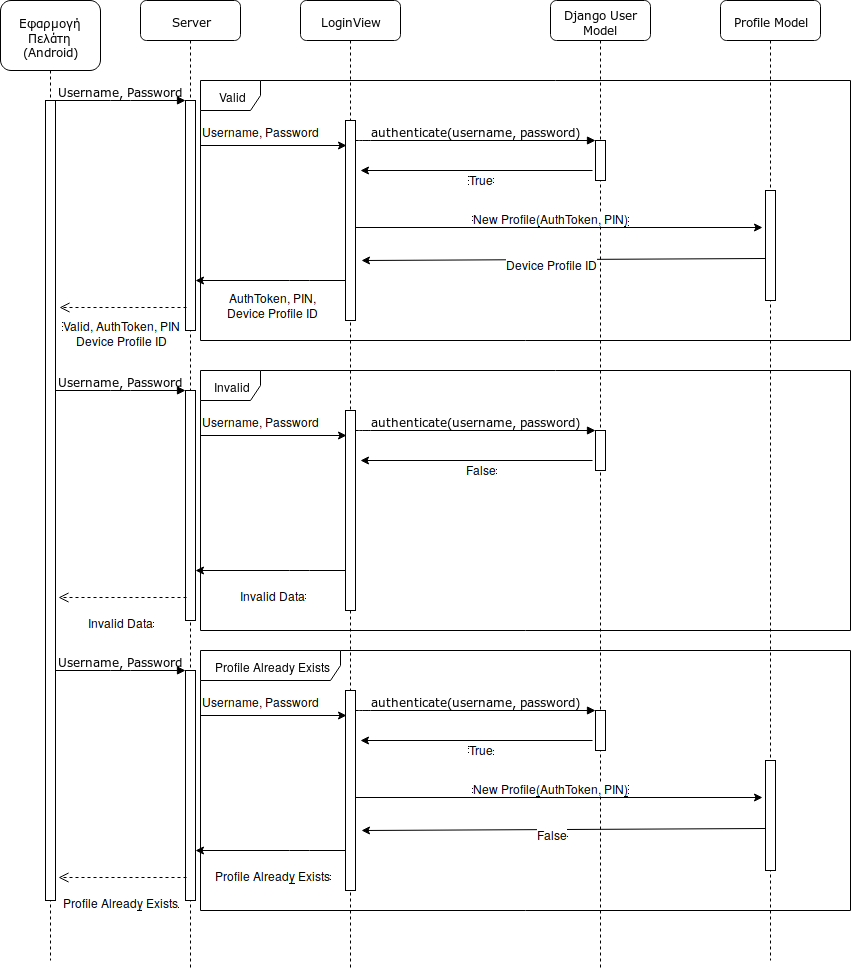
\includegraphics[width=\textwidth,height=\textheight,keepaspectratio]{LoginView_Sequence.png}
			\caption{Στάδιο Εισόδου}
			\label{fig:login_stage}
		\end{figure}

	\subsection{Στάδιο Ξεκλειδώματος - Unlock}
		Από την στιγμή που μια συσκευή αποκτήσει το δικό της προφίλ, και θεωρηθεί εξουσιοδοτημένη, μπορεί να αποστείλει αιτήματα ξεκλειδώματος.

		Αρχικά, ο χρήστης πληκτρολογεί στην εφαρμογή Android το 6ψήφιο προσωπικό του PIN και αγγίζει το κουμπί "Unlock". Ξεκινά η διαδικασία ξεκλειδώματος. Το πρώτο βήμα είναι να ανακτηθεί το Auth Token από τα Shared Preferences της συσκευής (σε κρυπτογραφημένη μορφή) και να αποκρυπτογραφηθεί με χρήση του Android Keystore. Αφότου αποκρυπτογραφηθεί, αποστέλει η εφαρμογή Android το Auth Token, τον αριθμό προφίλ της συσκευής και το PIN που πληκτρολόγησε ο χρήστης, στον Server.

		Ο Server λαμβάνει και τα τρία και πραγματοποιεί αναζήτηση για κάποιο προφίλ με αυτόν τον αριθμό προφίλ συσκευής που έλαβε. Αν υπάρχει, γίνεται επαλήθευση του Auth Token και του PIN που δώθηκαν. Αν επαληθεύονται επιτυχώς, γίνεται ενεργοποίηση του μηχανισμού ξεκλειδώματος και στέλνεται απάντηση (response) επιτυχίας στην συσκευή. Αν δεν επαληθεύονται στέλνεται απάντηση αποτυχίας.

		Αν δεν υπάρχει προφίλ με αυτό τον αριθμό, και πάλι η διαδικασία σταματάει με αποτυχία. Και στις δύο περιπτώσεις (επιτυχίας, αποτυχίας), γίνεται καταγραφή της απόπειρας πρόσβασης στο ημερολόγιο πρόσβασης του συστήματος.

		\begin{figure}[h]
			\centering
				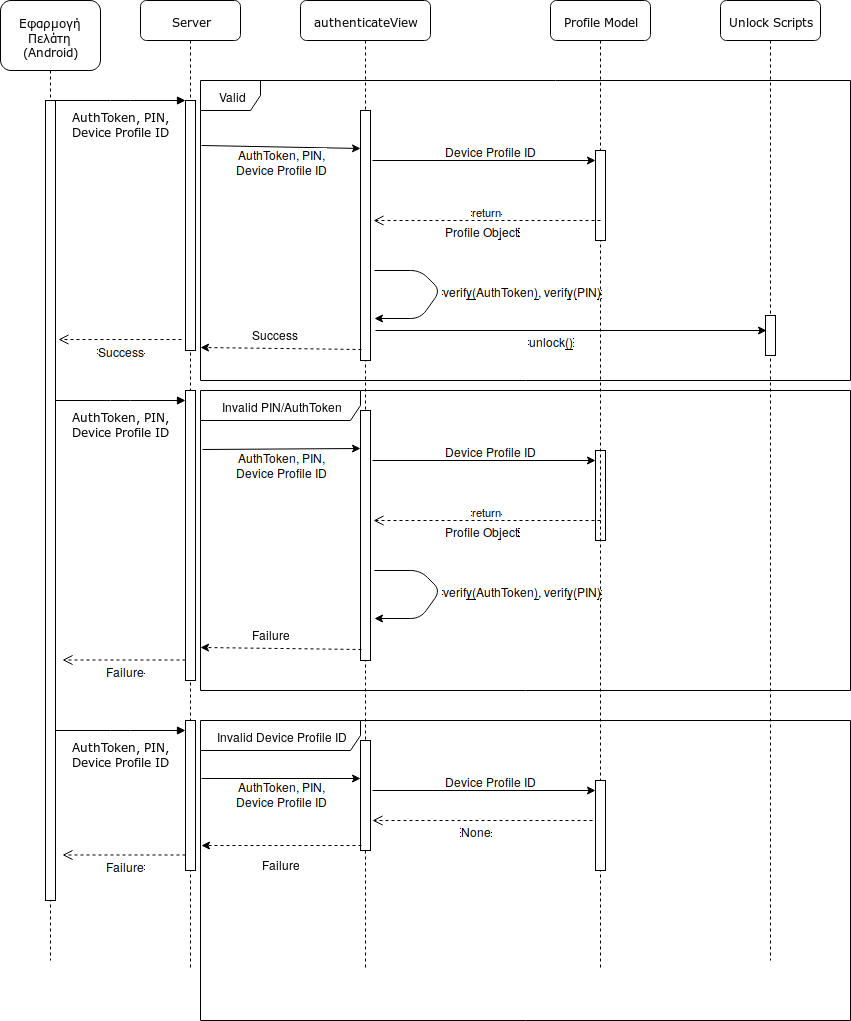
\includegraphics[width=\textwidth,height=\textheight,keepaspectratio]{UnlockView_Sequence.png}
			\caption{Στάδιο Ξεκλειδώματος}
			\label{fig:unlock_stage}
		\end{figure}

	\subsection{Ξεκλείδωμα μέσω Android Wear - Wear Unlock}
		\label{subsec:wear_unlock}
		Προκειμένου να γίνει εφικτό να γίνονται αιτήματα ξεκλειδώματος μέσω Android Wear κατά βούληση, θα πρέπει να γίνει πρώτα ένας "συγχρονισμός" με την Android Wear συσκευή. Προκειμένου να γίνει αυτός ο συγχρονισμός, απαιτείται η συσκευή να είναι εξουσιοδοτημένη (να έχει περάσει επιτυχώς το στάδιο εισόδου).

		Αφότου ο χρήστης πληκτρολογήσει το PIN του στην κεντρική οθόνη ξεκλειδώματος της εφαρμογής Android, μέσω ενός πλήκτρου που υπάρχει στο μενού του Action Bar, μπορεί να ζητήσει να γίνει συγχρονισμός με την Android Wear συσκευή του. Με το κλικ σε αυτό το πλήκτρο, αποστέλλεται αίτημα γέννησης τεκμηρίου εξουσιοδότησης Android Wear (βλ. \fullref{sec:models}) στον Server.

		Ο Server λαμβάνει το αίτημα αυτό, στο οποίο εμπεριέχονται το Auth Token της συσκευής, ο αριθμός προφίλ συσκευής και το PIN του χρήστη. Αφότου γίνει επαλήθευση των στοιχείων αυτών, παράγεται τυχαία ένα αλφαριθμητικό 30 χαρακτήρων γνωστό ως Wear Token, αποθηκεύεται hashed στο προφίλ της συσκευής, στην ΒΔ, και αποστέλλεται στην συσκευή Android. Αφότου παραληφθεί από την συσκευή Android γίνεται αποστολή του Wear Token στην συσκευή Android Wear. Πλέον μπορούν να γίνουν αιτήματα ξεκλειδώματος μέσω Android Wear.

		Όταν αιτείται ξεκλείδωμα μέσω Android Wear, γίνεται αποστολή του Wear Token (που βρίσκεται στο Smartwatch) και του Auth Token (που βρίσκεται στο Smartphone) στον Server και γίνεται ταυτοποίησή τους. Αν αντιστοιχούν σε υπάρχον προφίλ συσκευής, γίνεται ενεργοποίηση του μηχανισμού ξεκλειδώματος.

		Εάν κατα κάποιο σημείο αποτύχει κάποια επαλήθευση, γίνεται αποστολή μηνύματος αποτυχίας στην συσκευή Android.

	\subsection{Αλλαγή PIN χρηστών}
		Όπως αναφέρθηκε προηγουμένως (\fullref{sec:pilock_client_overview}), μία από τις λειτουργίες της εφαρμογής πελάτη για Android είναι η δυνατότητα αλλαγής του προσωπικού PIN του χρήστη, εφόσον το επιθυμεί. Για να γίνει αυτό ακολουθείται μια παρόμοια διαδικασία με αυτή του δεύτερου σταδίου εξουσιοδότησης πρόσβασης.

		Ο χρήστης υποχρεούται να πληκτρολογήσει το παλιό του PIN, μαζί με το νέο. Μόλις γίνει η πληκτρολόγηση, αποστέλλεται στον Server ένα αίτημα αλλαγής PIN με το παλιό και το νέο PIN, το Auth Token και το νούμερο προφίλ συσκευής. Ο Server τα επιβεβαιώνει, και εφόσον είναι επιτυχής η επιβεβαίωση, γίνεται αλλαγή του PIN στο νέο, που επιθυμεί ο χρήστης. Εαν τα στοιχεία που δώθηκαν δεν είναι έγκυρα, γίνεται απόρριψη του αιτήματος.

	\subsection{Ασφάλεια}
		Το σύστημα που αναλύθηκε παραπάνω έχει δημιουργηθεί με την ασφάλεια κατά νου. Για αυτόν τον λόγο δεν επιτρέπεται να γίνει αίτημα ξεκλειδώματος από μή εξουσιοδοτημένες συσκευές. Πρέπει \textbf{υποχρεωτικά} μία συσκευή να περάσει από το πρώτο στάδιο πριν να αποπειραθεί να κάνει αίτημα ξεκλειδώματος.

		Αν ένας χρήστης με κακόβουλες προθέσεις επιλέξει να παραλήψει το πρώτο στάδιο, για να μπορέσει να πραγματοποιήσει ξεκλείδωμα θα πρέπει πρωτίστος να καταφέρει να "μαντέψει" το Auth Token, είτε μαντεύοντας το Auth Token, είτε δοκιμάζοντας όλους τους δυνατούς συνδυασμούς χαρακτήρων προκειμένου να βρεθεί το σωστό Auth Token. Και στις 2 περιπτώσεις, είναι εξαιρετικά δύσκολο να βρεθεί το Auth Token. Στην περίπτωση που ο χρήστης επιλέξει να μαντέψει το Auth Token, εκμεταλλευόμενος την γεννήτρια τυχαιότητας, είναι αδύνατον να μαντέψει το αποτέλεσμα της συνάρτησης σε μία συγκεκριμένη στιγμή, καθώς χρησιμοποιείται η βέλτιστη πυγή τυχαιότητας του λειτουργικού συστήματος την συγκεκριμένη στιγμή μέσω της κλάση \verb|SystemRandom| της Python, η οποία εγγυάται ασφαλή τυχαιότητα. 

		Στην περίπτωση που ο κακόβουλος χρήστης επιλέξει να μαντέψει το Auth Token εξαντλώντας όλους τους πιθανούς συνδυασμούς χαρακτήρων, λόγω του μεγέθους και της πολυπλοκότητας του Auth Token (50 χαρακτήρες, μικρά γράμματα, σύμβολα), θα πρέπει να δοκιμάσει κατά μέσο όρο \(50^{50}/2=\sim4,440892098×10^{84}\) πιθανούς συνδυασμούς χαρακτήρων (με επαναλήψεις). Παρομοίως, για το Wear Token, θα χρειαστεί να εκτελέσει, κατά μέσο όρο \(50^{32}/2=\sim1,164153218×10^{54}\) πιθανούς συνδυασμούς χαρακτήρων (με επαναλήψεις). Αυτό καθιστά πολύ δύσκολο να σπάσει κάποιο από τα δύο tokens, με αποτέλεσμα να είναι σχεδόν αδύνατον να εισβάλλει κάποιος στο σύστημα. Σε αυτό το σημείο αξίζει να προστεθεί οτι προκειμένου ο εξυπηρετητής να εγκρίνει το αίτημα ξεκλειδώματος χρειάζεται να μαντέψει ο κακόβουλος χρήστης, παράλληλα με το Auth Token, και το PIN του χρήστη. Ο εξυπηρετητής δεν διαφοροποιεί τις απαντήσεις του προς την εφαρμογή πελάτη αν είναι σωστό ένα εκ των δύο στοιχείων πρόσβασης, δηλαδή δεν θα δώσει κάποιο στοιχείο ως προς το τι είναι λανθασμένο. Πρέπει να είναι και τα δύο στοιχεία σωστά προκειμένου να εγκριθεί το αίτημα και στην συγκεκριμένη περίπτωση, το να μαντέψει κάποιος το Auth Token \textbf{παράλληλα} με το PIN του χρήστη είναι εξαιρετικά δύσκολο.

		Τέλος, η διεξαγωγή της μεταφοράς δεδομένων από τον Server προς την εφαρμογή πελάτη γίνεται με κρυπτογράφηση SSL και όπως θα δούμε αργότερα, στο σχετικό κεφάλαιο, γίνεται κλείδωμα του πιστοποιητικού που χρησιμοποιείται στην εφαρμογή πελάτη, προκειμένου να είναι αδύνατον να γίνει παραχάραξη του. Προκειμένου, επίσης, να αποτρέψουμε επιθέσεις τύπου Protocol Downgrading, χρησιμοποιείται HSTS (HTTP Strict Transfer Security)\sucite{hsts}. 

\section{Λειτουργία Heartbeat}
	\label{sec:heartbeat}
	Προκειμένου να μπορούμε, με κάποιο τρόπο να διακρίνουμε αν ο Server είναι ενεργός, έπρεπε να υλοποιηθεί ένας μηχανισμός αναφοράς κατάστασης. Αυτός ο μηχανισμός είναι γνωστός ως Heartbeat, στην περίπτωση του PiLock. Αποτελείται από μία σελίδα στην οποία, όπως και στο υπόλοιπο API, χρησιμοποιείται JSON, προκειμένου να αναφέρει την έκδοση του Server, καθώς επίσης και την κατάσταση του Server (\autoref{fig:heartbeat}). 

	\begin{figure}[h]
	\centering
		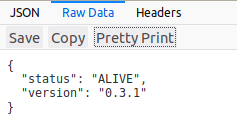
\includegraphics{heartbeat.png}
	\caption{Μήνυμα Heartbeat}
	\label{fig:heartbeat}
	\end{figure}

	Το Heartbeat χρησιμοποιείται προκειμένου να μπορέσει να αντιληφθεί η εφαρμογή Android αν το σύστημα είναι ενεργό, πριν να αποστείλλει κάποιο αίτημα ξεκλειδώματος. Χρησιμοποιείται επίσης και για να λειτουργήσει ο γενικός διακόπτης, όπως θα αναλυθεί παρακάτω. Η έκδοση του λογισμικού του Server μεταδίδεται προκειμένου να γνωρίζουμε εάν η εφαρμογή πελάτη είναι ενημερωμένη ώστε να μπορεί να λειτουργήσει με την παρούσα έκδοση λογισμικού στον Server. 

\section{Γενικός Διακόπτης}
	Πολλές φορές καθίσταται αναγκαίο να υπάρχει ένας γενικός διακόπτης, προκειμένου να αποκλείει αυτόματα οποιαδήποτε απόπειρα ξεκλειδώματος ή πρόσβασης στο σύστημα του PiLock. Αυτό καθίσταται ιδιαίτερα χρήσιμο σε περιπτώσεις που έχει συμβεί κάποιο εξαιρετικά σημαντικό συμβάν και να χρειάζεται να διακόψουμε την οποιαδήποτε πρόσβαση σε οποιονδήποτε χρήστη. 

	Για να υλοποιηθεί αυτό, δημιουργήθηκε ένα αρχείο διαμόρφωσης σε γλώσσα σήμανσης YAML, γνωστό ως \verb|config.yml| το οποίο τοποθετείται στον αρχικό κατάλογο του Project κατά την εγκατάσταση. Μέσα σε αυτό υπάρχει η εξής μεταβλητή:

	\begin{lstlisting}
	enabled: True\end{lstlisting}

	Εαν η μεταβλητή αλλάξει από τον χρήστη σε False, αυτόματα πλέον το μήνυμα που μεταδίδεται κατά την διαδικασία του Heartbeat αλλάζει. Συγκεκριμένα, πλέον η κατάσταση που μεταδίδει το Heartbeat αλλάζει σε \verb|status="LOCKED"|. Αυτό σηματοδοτεί την εφαρμογή πελάτη να ακυρώσει την διαδικασία που προτάθηκε από τον χρήστη, εφόνον λάβει αυτό το μήνυμα.